\section{RQ2: Hybrid Key Exchange on Federal \texttt{.gov}}
\label{sec:rq2}

\subsection{Method}

\paragraph{Targets.} CISA publishes the list of registered federal
\texttt{.gov} domains with their branch and agency~\cite{dotgovdata}. We took
all \data{rqtwo-domains} domains at commit \texttt{\data{rqtwo-dotgov-commit}}
and probed the two names a visitor types, the apex and \texttt{www.}, on port
443: \data{rqtwo-endpoints} endpoints. The list holds registered domains, so
services on other names (\texttt{login.}, \texttt{api.}, agency subdomains)
are outside the sample.

\paragraph{Probe.} On \data{rqtwo-date}, between \data{rqtwo-scan-start} and
\data{rqtwo-scan-end} UTC, \tool{} sent each endpoint its TLS~1.3 ClientHello,
offering X25519MLKEM768, X25519 and P-256 with key shares for the first two as
Go's default client does, and read the ServerHello. It then made a
standard \texttt{crypto/tls} handshake for the certificate chain and TLS
version. The global rate was \data{rqtwo-rate} connections per second from a
single vantage point, a consumer Internet connection, with the limits of
\S\ref{sec:design}.

\paragraph{Classification.} An endpoint is \emph{hybrid} if the ServerHello
or HelloRetryRequest selected a hybrid group, \emph{classical} if it selected a
classical group, and \emph{TLS~1.2 or lower} if there was no TLS~1.3
ServerHello but the standard handshake succeeded at a lower version. The
remaining endpoints did not resolve, did not accept a TCP connection, or
failed both handshakes. Adoption is the share of hybrid endpoints among those
that speak TLS, with a Wilson 95\% interval~\cite{wilson1927}. A domain takes
the better status of its two endpoints. Each endpoint's autonomous system (AS)
comes from the address probed, mapped with the iptoasn table dated
\data{rqtwo-asn-date}~\cite{iptoasn}.

\paragraph{Cross-check.} Both clients offer X25519MLKEM768, so on the
\data{rqtwo-xcheck-both} endpoints where both reached a group, the
independent \texttt{crypto/tls} handshake checks the hand-built probe. They
agree on hybrid versus classical for \data{rqtwo-xcheck-class} of them and on
the exact group for \data{rqtwo-xcheck-group}; the other
\data{rqtwo-xcheck-unoffered} servers picked P-384 or P-521, which only
\texttt{crypto/tls} offered.

\subsection{Results}

Of the \data{rqtwo-endpoints} endpoints, \data{rqtwo-ep-unresolvable} did not
resolve in DNS, \data{rqtwo-ep-unreachable} refused or dropped TCP connections
on port 443, and \data{rqtwo-ep-tls-error} accepted a connection but completed
no handshake, leaving \data{rqtwo-ep-responding} that speak TLS.

\paragraph{Adoption.} \data{rqtwo-ep-hybrid} of the
\data{rqtwo-ep-responding} TLS endpoints negotiated a hybrid group: an
adoption of \data{rqtwo-ep-share} (95\% CI \data{rqtwo-ep-ci}). At the domain
level, \data{rqtwo-dom-hybrid} of \data{rqtwo-dom-responding} domains
(\data{rqtwo-dom-share}, CI \data{rqtwo-dom-ci}) have at least one hybrid
endpoint. Every hybrid endpoint chose \data{rqtwo-hybrid-groups}, and
\data{rqtwo-hello-retry} reached it through a HelloRetryRequest. No endpoint
chose a pure post-quantum group. Of the rest, \data{rqtwo-ep-classical}
(\data{rqtwo-ep-classical-share} of TLS endpoints) speak TLS~1.3 but chose a
classical group, and \data{rqtwo-ep-tls1-2-or-lower}
(\data{rqtwo-ep-tlstwelve-share}) do not speak TLS~1.3 at all, so they cannot
negotiate a hybrid group without a software upgrade. Among endpoints that
speak TLS~1.3, adoption is \data{rqtwo-ep-hybrid-of-tlsthirteen}.

By branch, adoption is \data{rqtwo-ep-exec-share} for the executive branch
(\data{rqtwo-ep-exec-responding} TLS endpoints),
\data{rqtwo-ep-leg-share} for the legislative
(\data{rqtwo-ep-leg-responding}) and \data{rqtwo-ep-jud-share} for the
judicial (\data{rqtwo-ep-jud-responding}).

\begin{figure}[t]
\centering
% Generated by paper/gen.py from paper/data. Do not edit.
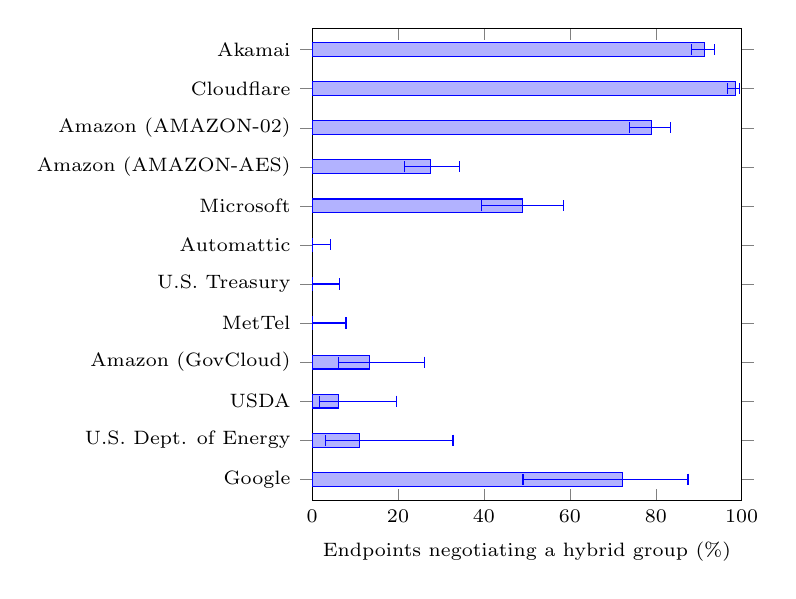
\begin{tikzpicture}
\begin{axis}[
  xbar, xmin=0, xmax=100, scale only axis, width=0.45\linewidth, height=6cm,
  xlabel={Endpoints negotiating a hybrid group (\%)},
  ytick={0,...,11},
  yticklabels={{Google},{U.S. Dept. of Energy},{USDA},{Amazon (GovCloud)},{MetTel},{U.S. Treasury},{Automattic},{Microsoft},{Amazon (AMAZON-AES)},{Amazon (AMAZON-02)},{Cloudflare},{Akamai}},
  y tick label style={font=\scriptsize}, x tick label style={font=\scriptsize},
  label style={font=\scriptsize}, bar width=5pt, enlarge y limits=0.05,
]
\addplot+[error bars/.cd, x dir=both, x explicit] coordinates {
  (72.2,0) += (15.3,0) -= (23.1,0)
  (11.1,1) += (21.7,0) -= (8.0,0)
  (6.1,2) += (13.5,0) -= (4.4,0)
  (13.3,3) += (12.8,0) -= (7.1,0)
  (0.0,4) += (7.9,0) -= (0.0,0)
  (0.0,5) += (6.3,0) -= (0.0,0)
  (0.0,6) += (4.3,0) -= (0.0,0)
  (49.0,7) += (9.6,0) -= (9.5,0)
  (27.5,8) += (6.8,0) -= (5.9,0)
  (79.1,9) += (4.4,0) -= (5.2,0)
  (98.6,10) += (0.8,0) -= (1.9,0)
  (91.4,11) += (2.3,0) -= (3.0,0)
};
\end{axis}
\end{tikzpicture}

\caption{Hybrid adoption among TLS endpoints in the
\data{rqtwo-asn-topk} autonomous systems hosting the most, with Wilson
95\% intervals.}
\label{fig:rq2-asn}
\end{figure}

\begin{table*}[t]
\centering\small
% Generated by paper/gen.py from paper/data. Do not edit.
\begin{tabular}{p{0.40\linewidth}rrrrrr}
\toprule
Autonomous system & TLS & Hyb. & Cl. & $\le$1.2 & Share & 95\% CI \\
\midrule
AS20940 Akamai International B.V. & 431 & 394 & 0 & 37 & 91.4\% & 88--94 \\
AS13335 Cloudflare, Inc. & 346 & 341 & 0 & 5 & 98.6\% & 97--99 \\
AS16509 Amazon (AMAZON-02) & 277 & 219 & 46 & 12 & 79.1\% & 74--83 \\
AS14618 Amazon (AMAZON-AES) & 189 & 52 & 110 & 27 & 27.5\% & 22--34 \\
AS8075 Microsoft Corporation & 102 & 50 & 26 & 26 & 49.0\% & 40--59 \\
AS2635 Automattic, Inc & 85 & 0 & 85 & 0 & 0.0\% & 0--4 \\
AS13506 U.S. Treasury & 57 & 0 & 6 & 51 & 0.0\% & 0--6 \\
AS16524 MetTel & 45 & 0 & 37 & 8 & 0.0\% & 0--8 \\
AS8987 Amazon (GovCloud) & 45 & 6 & 36 & 3 & 13.3\% & 6--26 \\
AS4155 USDA & 33 & 2 & 3 & 28 & 6.1\% & 2--20 \\
AS32982 U.S. Dept. of Energy & 18 & 2 & 5 & 11 & 11.1\% & 3--33 \\
AS396982 Google LLC & 18 & 13 & 5 & 0 & 72.2\% & 49--88 \\
\midrule
other 77 ASes & 314 & 51 & 130 & 133 & 16.2\% &  \\
\bottomrule
\end{tabular}

\caption{TLS endpoints by autonomous system: those that negotiated a hybrid
group (Hyb.), a classical TLS~1.3 group (Cl.) or no TLS~1.3 ($\le$1.2), for
the \data{rqtwo-asn-topk} ASes hosting the most, which hold
\data{rqtwo-asn-topk-cover} of TLS endpoints.}
\label{tab:rq2-asn}
\end{table*}

\paragraph{The provider decides.} Concurrent measurements of the wider web
found that managed infrastructure providers drive post-quantum
deployment~\cite{wickramasinghe2026} and that the provider predicts it
better than the organization's sector~\cite{loizou2026}. The federal web shows
the same pattern. Figure~\ref{fig:rq2-asn} and
Table~\ref{tab:rq2-asn} break adoption down by AS. Endpoints are
concentrated: the two largest ASes, Akamai and Cloudflare, hold
\data{rqtwo-top2-cover} of TLS endpoints and \data{rqtwo-top2-hybrid-cover}
of hybrid ones. Adoption there is \data{rqtwo-as20940-share} (Akamai) and
\data{rqtwo-as13335-share} (Cloudflare), and Fastly's
\data{rqtwo-as54113-n} endpoints are all hybrid. Large clouds sit in the
middle and differ by service: \data{rqtwo-as16509-share} on Amazon's main AS
but \data{rqtwo-as14618-share} on its AMAZON-AES AS and
\data{rqtwo-as8987-share} on GovCloud; \data{rqtwo-as8075-share} on Microsoft.
At the other end, none of the \data{rqtwo-as2635-n} endpoints hosted by
Automattic, the \data{rqtwo-as16524-n} on MetTel or the
\data{rqtwo-as13506-n} on the Treasury's own network negotiated a hybrid
group; on the Treasury's network \data{rqtwo-as13506-tlstwelve} of them do
not speak TLS~1.3.

What the federal population adds is the agency, the unit that M-26-15 holds
responsible for migration. To test whether the provider or the agency better
predicts the outcome, we
apply one rule to both groupings: among groups with at least
\data{rqtwo-uniform-min} TLS endpoints, what share of endpoints sit in a
group that is nearly uniform, with adoption at most \data{rqtwo-uniform-lo}
or at least \data{rqtwo-uniform-hi}? For ASes it is
\data{rqtwo-uniform-as-share} of endpoints (\data{rqtwo-uniform-as-groups}
ASes); for agencies, \data{rqtwo-uniform-agency-share}
(\data{rqtwo-uniform-agency-groups} agencies). Agencies are mixtures of
providers; providers are mostly all-or-nothing. Adoption among agencies with
at least \data{rqtwo-agency-min} TLS endpoints
(Table~\ref{tab:rq2-agencies} in the appendix) ranges from
\data{rqtwo-agency-min-share} to \data{rqtwo-agency-max}.

\paragraph{Certificates.} Post-quantum key exchange protects confidentiality
only; authentication is still classical everywhere. Of the
\data{rqtwo-cert-endpoints} TLS endpoints whose leaf certificate we recorded,
\data{rqtwo-cert-rsa-share} use RSA keys (\data{rqtwo-cert-rsa2048-share}
RSA-2048) and \data{rqtwo-cert-ecdsa-share} ECDSA keys; no other key type
appears.

\paragraph{Limits.} One vantage point and one moment: CDNs answer from the
edge nearest the scanner, and results may differ by location and over time.
The probe connects to the first resolved address, so a name served by two
providers is measured at one. A server that supports a hybrid group but
prefers X25519 when both are offered counts as classical, which is what a
browser would negotiate with it. We do not measure server software, which
would require an HTTP request beyond the handshake; the AS identifies the
hosting provider, not the software.
